\section{Diseño experimental}
\label{sec:diseno}
En la fase de selección de características, utilizamos seis esquemas de preprocesamiento distintos. Estos esquemas se basan en la combinación de medidas de relevancia y similitud, implementadas dentro del marco propuesto por \cite{liu_empirical_2015}. Cada esquema de preprocesamiento se integra con el modelo de clasificación de RF para evaluar su eficacia utilizando el conjunto de datos BugHunter.

\subsubsection{Esquemas de Preprocesamiento}

Los seis esquemas diseñados se detallan a continuación:

\begin{enumerate}
    \item \textbf{IG + SU:} Se utiliza para el análisis de relevancia el algoritmo Ganancia de información y luego con las características resultantes se continua con el control de redundancia utilizando Incertidumbre simétrica.
    \item \textbf{CS + SU:} Se utiliza para el análisis de relevancia el algoritmo Chi-Cuadrado  y luego con las características resultantes se continua con el control de redundancia utilizando Incertidumbre simétrica.
    \item \textbf{RF + SU:} Se utiliza para el análisis de relevancia el algoritmo ReliefF y luego con las características resultantes se continua con el control de redundancia utilizando Incertidumbre simétrica.
    \item \textbf{IG + COS:} Se utiliza para el análisis de relevancia el algoritmo Ganancia de información y luego con las características resultantes se continua con el control de redundancia utilizando Semejanza de coseno.
    \item \textbf{CS + COS:} Se utiliza para el análisis de relevancia el algoritmo Chi-Cuadrado y luego con las características resultantes se continua con el control de redundancia utilizando Semejanza de coseno.
    \item \textbf{RF + COS:} Se utiliza para el análisis de relevancia el algoritmo ReliefF y luego con las características resultantes se continua con el control de redundancia utilizando Semejanza de coseno.
\end{enumerate}

Cada esquema se aplica al modelo de clasificación RF para demostrar su impacto en la eficacia de la selección de características en diferentes conjuntos de datos.

\subsubsection{Evaluación de Esquemas en el Modelo RF}

La evaluación de los esquemas se lleva a cabo mediante la integración con el modelo de clasificación RF. El objetivo es observar el rendimiento de cada esquema en términos de precision, recall y F-Measure al procesar los conjuntos de datos de BugHunter. Estos resultados ayudarán a determinar la efectividad de las combinaciones de medidas de relevancia y similitud en la etapa de selección de características.

\subsubsection{Descripción del flujo}
La figura \ref{fig:Flow} se divide en dos pasos: el \textbf{Paso 1}, de selección de características (\textit{Step 1: Features Selection} en la figura), y el \textbf{Paso 2}, de modelos de clasificación (\textit{Step 2: Classification Models}). El \textbf{Step 1} realiza la selección de características combinando análisis de relevancia (IG, CS y RF) y control de redundancia (SU, COS), teniendo como resultado un filtro del las características en los conjuntos de datos ingresados. El \textbf{Step 2} inicia dividiendo el conjunto de datos resultante del \textbf{Step 1} en entrenamiento y prueba, se mantiene un conjunto de entrenamiento original mientras se crea una copia pero balanceo el atributo clase utilizando diferentes técnicas (ROS,RUS y SMOTE) y luego se ingresan al algoritmo de clasificación quedando guardados los resultados de cada algoritmo en base de datos. 

La clasificación de características se usa para implementar el análisis de relevancia, mientras que \textbf{NTC} se usa para implementar el control de redundancia. Para la selección de características, se combina el análisis de relevancia y el control de redundancia en búsqueda de reducir la cantidad de características sin afectar los resultados de los clasificadores  \cite{liu_empirical_2015}.

El flujo descrito en la Figura \ref{fig:Flow} se realiza en diferentes iteraciones, donde el \textbf{Step 1} se itera por \(proyecto \rightarrow nivel \rightarrow k \rightarrow \beta\), teniendo como resultado las métricas seleccionadas. El \textbf{Step 2} itera \(proyecto \rightarrow nivel \rightarrow k \rightarrow \beta \rightarrow modelosSeleccion \), donde el último nivel hace referencia a los esquemas utilizados para la selección de características del \textbf{Step 1}. Esto permite que el \textbf{Step 2} ejecute los algoritmos de clasificación solo con las métricas que se seleccionaron y almacene en la base de datos los resultados.

Siendo $k$ en el proceso de \textbf{análisis de relevancia} (\textit{relevance analysis}) el valor utilizado como ranking para seleccionar las características en dependencia del orden resultante de los algoritmos  \textbf{IG, CS y RF}. En el proceso siguiente, de \textbf{control de redundancia} (\textit{redundancy check}), \(\beta \) representa el umbral para discriminar cuales métricas quedaran seleccionadas por el algoritmo \textbf {NTC}. 
Ambos pasos son explicados en detalle en los algoritmos \ref{alg:featureSelection} y \ref{alg:executionmodels}.
\begin{enumerate}
\item Selección de características (\textit{Features Selection}):
\begin{enumerate}
\item \textbf{BugHunter:} conjunto de datos almacenado en archivos CSV estructurados con la jerarquía proyecto-nivel (método, clase y archivo). Por tanto, hay 15 proyectos y 3 archivos por proyecto, un total de 45 archivos, cada uno con las métricas respectivas a su nivel. Se incluye un repositorio adicional etiquetado como \textbf{ALL} que es la unión de los 15 proyectos por cada nivel.
\item \textbf{Discretización de la clase:} proceso en el que la variable de clase se transforma en categorías. La clase original del conjunto de datos contiene un valor numerico indicando la cantidad de errores encontrados en cada registro, al ser discretizado quedan solo dos clases sin errores o con errores.
\item \textbf{Análisis de relevancia:}  para este proceso se utilizan los algoritmos IG, CS y RF, los resultados de estos algoritmos para cada característica se filtran seleccionando las k características que superen los ranking 50\%, 70\% y 90\%.
\item \textbf{Control de redundancia:} se utiliza el algoritmo NTC con los métodos SU y COS. El algoritmo es aplicado a las características seleccionadas en el paso anterior ingresando un umbral \(\beta\) (0.5, 0.7 y 0.9) el cual se encuentra en un rango entre 0 y 1. Se seleccionan aquellas características que superen el umbral ingresado a NTC.
\end{enumerate}

\item Modelos de clasificación (\textit{Classification Models}):
\begin{enumerate}
\item \textbf{División del Conjunto de Datos:} en esta fase, se procede a dividir el conjunto de datos, el cual ya incluye las métricas filtradas, en dos segmentos distintos: un \(33\%\) para el conjunto de pruebas y el \(67\%\) restante para el conjunto de entrenamiento. Para ello, se emplea la función \texttt{train\_test\_split} de la biblioteca \textit{scikit-learn} en Python. Se especifica el parámetro \texttt{stratify} con el fin de garantizar que las proporciones de las clases en los conjuntos de entrenamiento y pruebas sean representativas de las proporciones observadas en el conjunto de datos completo. Esta estrategia es crucial para mantener la consistencia y la validez estadística del proceso de validación del modelo.

\item \textbf{Balanceo de clases:} se aplican los algoritmos RUS, ROS y SMOTE para balancear la cantidad de registros con respecto a la clase. A modo de evitar que la etapa de pruebas se vea afectada por datos generados artificialmente solo se realiza el balanceo del conjunto de entrenamiento.
\item \textbf{Ejecución del modelo de clasificación:} para analizar la capacidad de los datos de predecir errores, se emplea el algoritmo de Random Forest (RF), descrito en la Sección \ref{sub:modelos}. Los conjuntos de entrenamiento y prueba generados en Python se exportan a archivos y el clasificador se ejecuta en Weka, en la modalidad \textit{Supplied test set}. Se ejecuta en dos instancias distintas para cada conjunto de datos que completa la etapa de selección de características: la primera utiliza un conjunto de entrenamiento balanceado y la segunda un conjunto sin balancear. Ambas ejecuciones comparten el mismo conjunto de pruebas para garantizar una comparación justa y coherente de los resultados.

\end{enumerate}
\end{enumerate}

\subsubsection{Orden de las etapas respecto de la partición entrenamiento/prueba}

El análisis de relevancia y el control de redundancia se calculan sobre el conjunto proyecto-nivel completo, es decir, antes de la partición en entrenamiento y prueba; el balanceo de clases, en cambio, se aplica exclusivamente dentro del conjunto de entrenamiento resultante. Dado que los tres algoritmos de relevancia (IG, CS y ReliefF) utilizan la etiqueta de clase de cada instancia, este orden introduce un riesgo de sesgo de selección: el subconjunto de características elegido puede estar influido por patrones presentes en instancias que después integrarán el conjunto de prueba \cite{ambroise2002,cawley2010}. Este riesgo afecta únicamente a la elección de qué columnas se conservan, y no a los parámetros del clasificador, que se ajustan solo con el conjunto de entrenamiento. Su magnitud se discute en el Capítulo \ref{cap:discusion}, y su corrección mediante un esquema de selección anidado se declara como trabajo futuro (Capítulo \ref{cap:conclusion}).

\subsubsection{Análisis de sensibilidad}

Para evaluar si los hallazgos dependen del clasificador, el flujo completo se repitió con \textit{Random Forest}, XGBoost y una SVM lineal, implementados en \textit{scikit-learn}, sobre la misma partición estratificada 67/33 con semilla fija y con los mismos subconjuntos de métricas. En este análisis se almacenan, además de las métricas agregadas, el \textit{F-measure} de la clase \textit{bug}, el MCC y el AUC-ROC de cada ejecución. Su diseño y resultados se presentan en la Sección \ref{sec:sensibilidad}.

\begin{figure}[H]
    \centering
    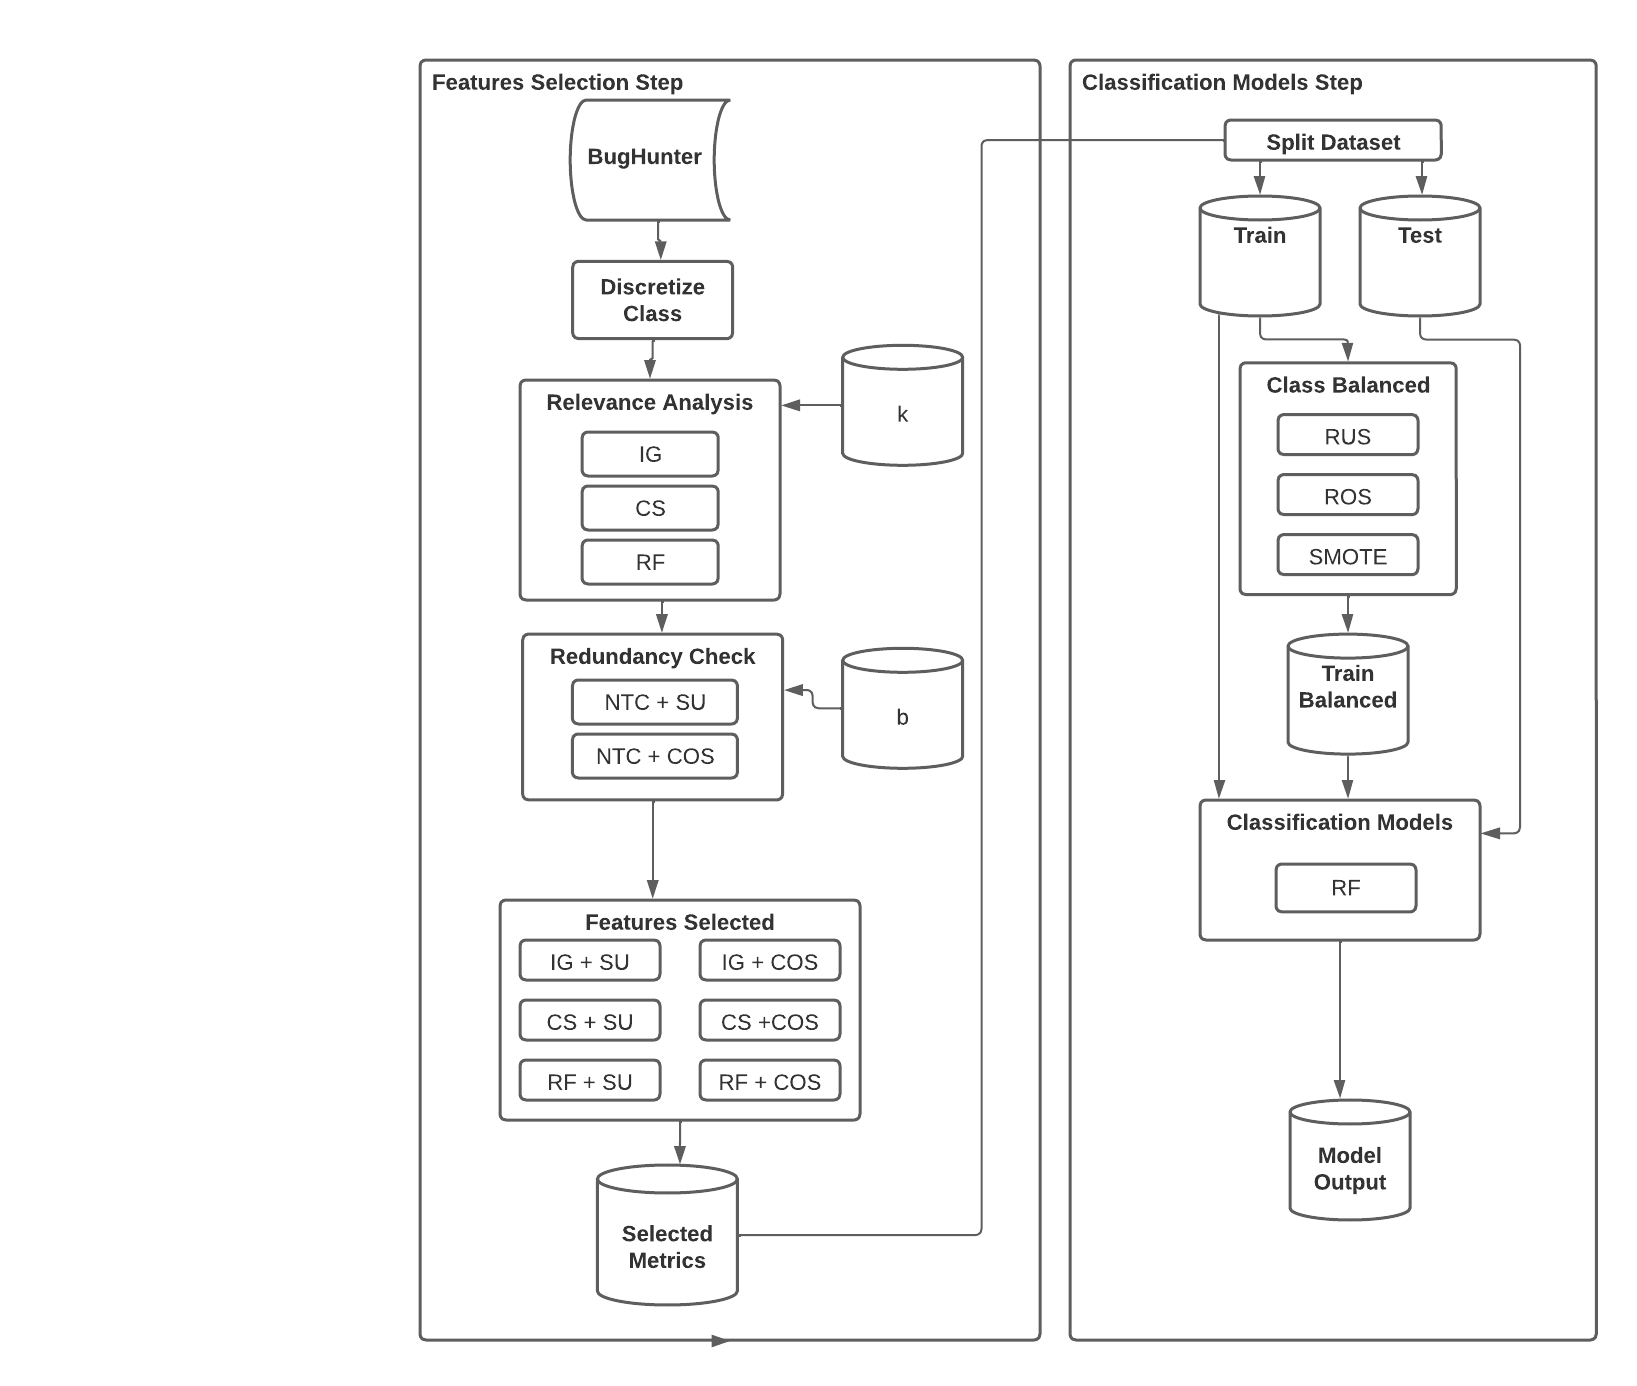
\includegraphics[width=150mm, height=110mm,]{figs/etapas/diagram.png}
    \captionsetup{labelsep=period, labelfont=bf}
    \setstretch{1} %Interlineado 1
    \caption{Descripción del flujo de trabajo}
    \label{fig:Flow}
\end{figure}

 El flujo descrito se ejecuta por cada proyecto iniciando con el proceso de selección de características. Cada proyecto contiene tres conjuntos de datos uno por cada nivel de métricas (Method, Class and File), el algoritmo \ref{alg:featureSelection} describe el primer paso del flujo \ref{fig:Flow}.
 
El algoritmo \ref{alg:featureSelection} describe el paso de Feature Selection. Se ejecuta ingresando cada conjunto de datos \(C_{p}(C_{\text{level}},C_{\text{class}},C_{\text{method}})\) donde \(_{p} \in \{p_{1},p_{2},...,p_{15}\}\) representa los 15 proyectos que contiene el BugHunter, y cada uno contiene tres conjuntos de datos, uno por cada nivel. Se guardan en la base de datos las métricas seleccionadas para cada nivel \(T_{\text{le}}(f_1,f_2,...,f_k)\) después de aplicar el análisis de relevancia y el control de redundancia. Utilizando tres ciclos anidados, se recorren las listas (\(rankList, bList, levelList\)) con la jerarquía \(rank \rightarrow \beta \rightarrow \text{level}\), donde \(rank\) se utiliza para seleccionar las métricas después del proceso de análisis de relevancia (IG, CS y RF), \(\beta\) es el umbral que se define para la ejecución del algoritmo NTC (análisis de redundancia), y \(\text{level}\) representa el nivel que se selecciona para el proyecto que se está analizando.

En cada iteración se lee el conjunto de datos (\(proyecto \rightarrow nivel\)) y se normaliza el atributo clase, dado que contiene valores numéricos que representan la cantidad de errores encontrados en esa medición, quedando solo con las clases BUG y NOBUG.

Se realiza el proceso de análisis de relevancia y el control de redundancia, y queda guardado en la base de datos qué métricas son seleccionadas en cada iteración y qué modelo de selección se utilizó, siendo este la combinación entre los algoritmos de relevancia y el control de redundancia. La lista queda como \(modelsSelections \rightarrow ['CS-SU','IG-SU','RF-SU','CS-COS','IG-COS','RF-COS']\).

 \begin{algorithm}[H]
    \hspace*{\algorithmicindent} \textbf{Input:} The original dataset $T_{le}(f_{1},f_{2},...,f_{k},l)$ where $l \in \{FP,NFP\}$ denotes the class label, and $k$ is the number of features. $le \in \{File, Class, Methods\}$ of a specific project

    \hspace*{\algorithmicindent} \textbf{Output:} Saves the selected characteristics in the Database. $T_{le}(f_1,f_2,...,f_k,l)$ where $k$ is the number of features selected by relevance analysis and redundancy check.
    \caption{Feature selection}
    \label{alg:featureSelection}
    \begin{algorithmic}[1]
    \fontsize{12pt}{12pt}\selectfont
    \REQUIRE $rankList \leftarrow [0.5, 0.7, 0.9]$
    \STATE $bList \leftarrow [0.5, 0.7, 0.9]$
    \STATE $levelList \leftarrow ['method', 'class', 'file']$
    \STATE $response \leftarrow \phi$

    \FOR{$\text{each}$ rank in $rankList$}
        \FOR{$\text{each}$ b in $bList$}
            \FOR{$\text{each}$ level in $levelList$}
                \STATE $data \leftarrow readDataset(level, project)$
                \STATE $data \leftarrow normalizeClass(data)$\;
                \STATE $square \leftarrow ChiSquare(data, rank)$\;
                \STATE $ig \leftarrow Ig(data, rank)$\;
                \STATE $relief \leftarrow ReliefF(data, rank)$\;
                \STATE $response \leftarrow response + NTC(b, square, 'CS-SU')$\;
                \STATE $response \leftarrow response + NTC(b, ig, 'IG-SU')$\;
                \STATE $response \leftarrow response + NTC(b, relief, 'RF-SU')$\;
                \STATE $response \leftarrow response + NTC(b, square, 'CS-COS')$\;
                \STATE $response \leftarrow response + NTC(b, ig, 'IG-COS')$\;
                \STATE $response \leftarrow response + NTC(b, relief, 'RF-COS')$\;
                \STATE $saveBD(response)$\;
            \ENDFOR
        \ENDFOR
    \ENDFOR
    \end{algorithmic}
\end{algorithm}

El algoritmo \ref{alg:executionmodels} representa el paso de modelos de clasificación. Se ingresan los mismos conjuntos de datos del algoritmo \ref{alg:featureSelection} pero $_{k}$ representa las métricas seleccionadas al ejecutar algoritmo \ref{alg:featureSelection}.

A los modelos de selección (\(modelsSelections\)) resultantes del algoritmo \ref{alg:executionmodels} se les agrega \(ALL\) que representa al conjunto de datos original sin realizar el paso de selección de características. Se agrega la lista de esquemas (\(modelsSelections\)) a los ciclos anidados. Quedando \(rank \rightarrow \beta \rightarrow level \rightarrow modelSelection\).

\begin{algorithm}[H]
    \hspace*{\algorithmicindent} \textbf{Input:} \\ The dataset $T_{le}(f_1, f_2, ..., f_k, l)$ where $l \in \{FP, NFP\}$ denotes the class label, and $k$ is the number of features selected by the feature selection process. $le \in \{File, Class, Methods\}$ of a specific project

    \hspace*{\algorithmicindent} \textbf{Output:} 
        Saves the precision, recall, accuracy, and f-measure in the Database 
    \caption{Execution of models}
    \label{alg:executionmodels}
    \begin{algorithmic}[1]
    \fontsize{12pt}{12pt}\selectfont
    \REQUIRE $rankList \leftarrow [0.5, 0.7, 0.9]$
    \STATE $rankList \leftarrow [0.5, 0.7, 0.9]$
    \STATE $bList \leftarrow [0.5, 0.7, 0.9]$
    \STATE $levelList \leftarrow ['method', 'class', 'file']$

    \STATE $modelsSelections \leftarrow ['CS-SU', 'IG-SU', 'RF-SU', 'CS-COS', 'IG-COS', 'RF-COS', 'ALL']$\;
    \STATE $response \leftarrow \phi$

    \FOR{$\text{each}$ rank in $rankList$}
        \FOR{$\text{each}$ b in $bList$}
            \FOR{$\text{each}$ level in $levelList$}
                \FOR{$\text{each}$ modelsSelection in $modelsSelections$}
                \STATE $data \leftarrow getData(rank, b, level, modelsSelection)$\;
                    \STATE $responseNormal \leftarrow ModelResult(data.original, model)$\;
                    \STATE $responseBalanced \leftarrow ModelResult(data.balanced, model)$\;
                    \STATE $saveBD(responseNormal)$\;
                    \STATE $saveBD(responseBalanced)$\;
                \ENDFOR
            \ENDFOR
        \ENDFOR
    \ENDFOR

    \end{algorithmic}
\end{algorithm}



En cada iteración se obtiene el conjunto de datos aplicando los filtros de métricas mencionados, este se utiliza para ejecutar los modelos de clasificación de la lista $models$. Los resultados de presision, recall y f-measure se almacenan en base de datos así como cada parámetro referente a la iteración para identificar a que conjunto de datos pertenecen y los parámetros de selección.



